\documentclass[12pt,aspectratio=169]{beamer}

\usetheme{metropolis}

\definecolor{mDarkBrown}{HTML}{FF5722}
\definecolor{mDarkTeal}{HTML}{263238}
\definecolor{mLightBrown}{HTML}{FF5722}

\usepackage{graphicx}
\usepackage{hyphenat}
\usepackage[normalem]{ulem}

\usepackage{minted}
\usemintedstyle{tango}

\usepackage{polyglossia}
\setdefaultlanguage[variant=british]{english}
\usepackage[english=british]{csquotes}

\defaultfontfeatures{Ligatures=TeX}
\setmainfont{Lucida Sans OT}
\setsansfont[Scale=MatchLowercase]{Lucida Sans OT}
\setmonofont[Scale=MatchLowercase]{Lucida Console DK}

\author{Gianluca Campanella}
\date{}



\title{Introduction to Data Science and Analytics}

\begin{document}

\maketitle

\begin{frame}{Before we start\ldots}
    \begin{center}
        \LARGE%
        \begin{tabular}{rl}
            SSID:     & \textbf{GA-Guest} \\
            Password: & \textbf{yellowpencil}
        \end{tabular}
    \end{center}
\end{frame}

\begin{frame}
    \begin{center}
        \LARGE%
        Welcome to \\[\medskipamount]
        \textbf{Introduction to} \\[\medskipamount]
        \textbf{Data Science and Analytics}
    \end{center}
\end{frame}

\begin{frame}{Contents}
    \tableofcontents[hideallsubsections]
\end{frame}

\section{What is Data Science?}

\begin{frame}{What is Data Science?}
    \only<1>{%
        \begin{columns}
            \begin{column}{0.5\textwidth}
                \begin{center}
                    Mathematics and \\ Statistics / Operational Research
                \end{center}
            \end{column}
            \begin{column}{0.5\textwidth}
                \begin{center}
                    Computing and \\ Software Engineering
                \end{center}
            \end{column}
        \end{columns}
        \vfill
        \begin{columns}
            \begin{column}{0.5\textwidth}
                \begin{center}
                    Visualisation and \\ Communication Skills
                \end{center}
            \end{column}
            \begin{column}{0.5\textwidth}
                \begin{center}
                    Domain expertise
                \end{center}
            \end{column}
        \end{columns}}
    \only<2>{%
        \begin{center}
            \LARGE%
            A \alert{problem\hyp{}solving approach} \\
            based on the scientific method
        \end{center}}
    \only<3>{%
        \vspace{0.5em}
        \begin{block}{Statistics}\vspace{-0.25em}
            \begin{itemize}
                \item Predates computers
                \item \alert{Understand why something happens} in the face of
                      uncertainty
            \end{itemize}
        \end{block}
        \vfill
        \begin{block}{Machine Learning}\vspace{-0.25em}
            \begin{itemize}
                \item `Algorithmic modelling' (L. Breiman)
                \item Computers can \alert{learn rules} without explicit
                      programming
            \end{itemize}
        \end{block}
        \vfill
        \begin{block}{Deep Learning}\vspace{-0.25em}
            \begin{itemize}
                \item Less structured inputs
                \item Computers can \alert{learn structure} without explicit
                      programming
            \end{itemize}
        \end{block}}
    \only<4>{%
        \begin{columns}[c]
            \begin{column}{0.25\textwidth}
            \end{column}
            \begin{column}{0.375\textwidth}
                \begin{center}
                    \Large\bf%
                    Predictions
                \end{center}
            \end{column}
            \begin{column}{0.375\textwidth}
                \begin{center}
                    \Large\bf%
                    Mechanisms
                \end{center}
            \end{column}
        \end{columns}
        \vfill
        \begin{columns}[c]
            \begin{column}{0.25\textwidth}
                \begin{center}
                    \Large\bf%
                    Analysis
                \end{center}
            \end{column}
            \begin{column}{0.375\textwidth}
                \begin{center}
                    \textbf{Descriptive} \\
                    What's happening?
                \end{center}
            \end{column}
            \begin{column}{0.375\textwidth}
                \begin{center}
                    \textbf{Diagnostic} \\
                    Why is it happening?
                \end{center}
            \end{column}
        \end{columns}
        \vfill
        \begin{columns}[c]
            \begin{column}{0.25\textwidth}
                \begin{center}
                    \Large\bf%
                    Building
                \end{center}
            \end{column}
            \begin{column}{0.375\textwidth}
                \begin{center}
                    \textbf{Predictive} \\
                    What's likely to happen?
                \end{center}
            \end{column}
            \begin{column}{0.375\textwidth}
                \begin{center}
                   \textbf{Prescriptive} \\
                   What do I need to do?
                \end{center}
            \end{column}
        \end{columns}}
    \only<5>{%
        \begin{block}{Data Science is\ldots}
            \begin{itemize}
                \setlength{\itemsep}{0.75em}
                \item \alert{Evidence\hyp{}based problem solving and
                             decision\hyp{}making}
                \item Multidisciplinary but domain\hyp{}driven
                \item Analysis\hyp{}focused or building\hyp{}focused
            \end{itemize}
        \end{block}}
\end{frame}

\section{Who is a Data Scientist?}

\begin{frame}{Who is a Data Scientist?}
    Someone who can\ldots
    \begin{itemize}
        \setlength{\itemsep}{0.75em}
        \item Get a `feel' for the data
        \item Communicate effectively
        \item Work well in a team
    \end{itemize}
\end{frame}

\begin{frame}{What's this `feel' for the data?}
    \only<1>{%
        \begin{itemize}
            \setlength{\itemsep}{0.75em}
            \item Passion for the domain
            \item Curiosity about the data
            \item Intuition and creativity
            \item Common sense
            \item Rigour and accuracy
            \item Relevance
        \end{itemize}}
    \only<2>{%
        \begin{center}
            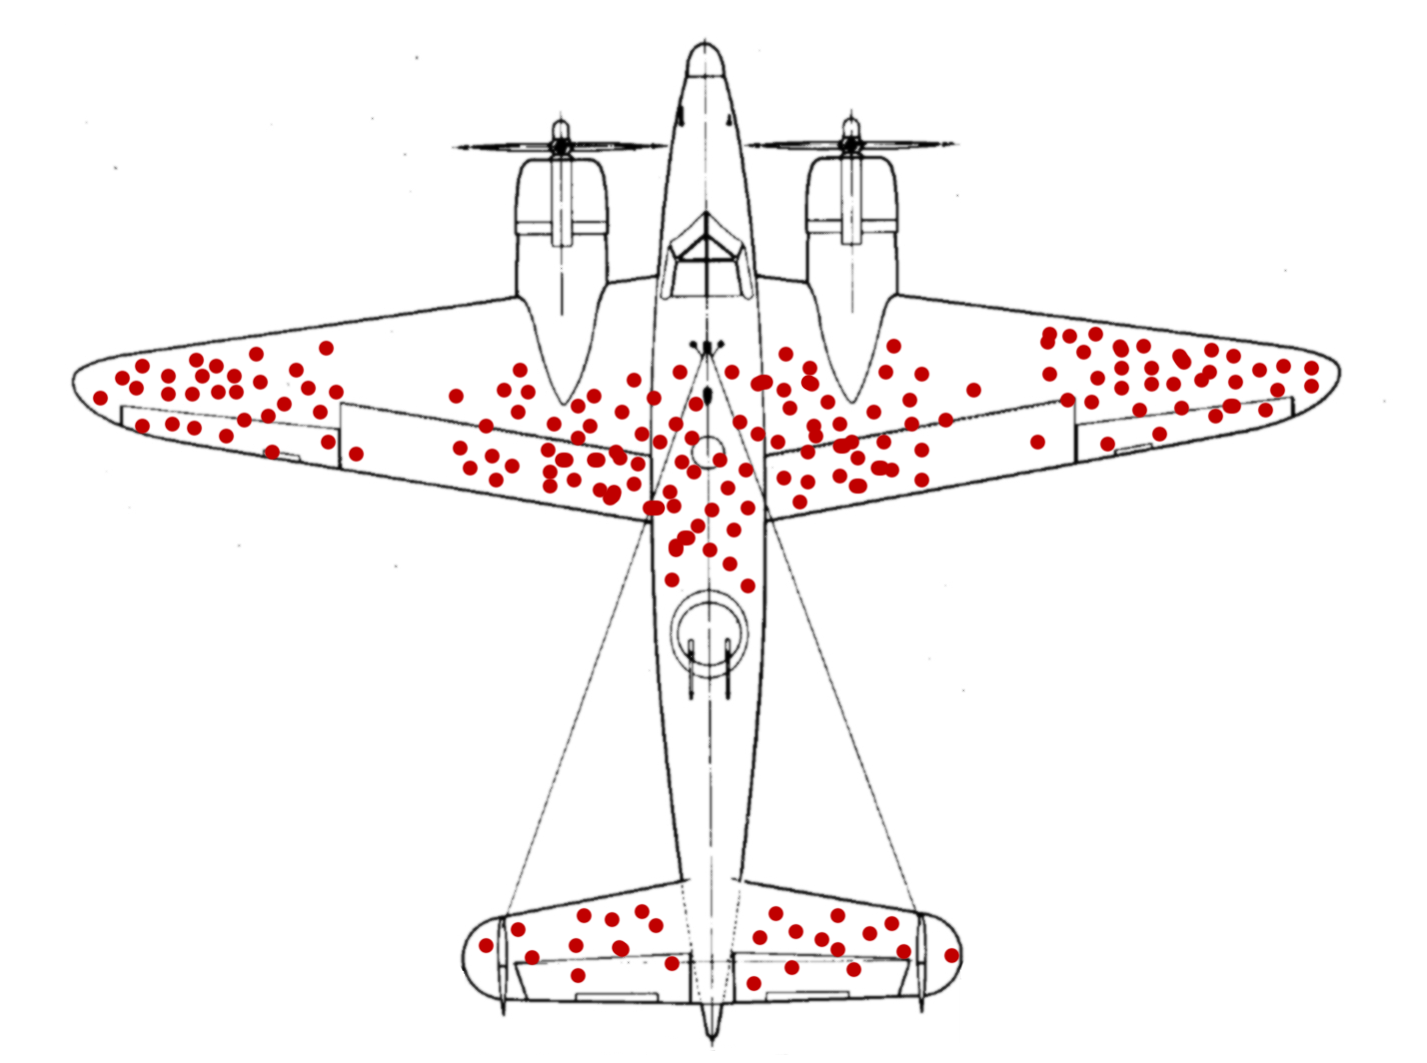
\includegraphics[height=0.8\textheight]{figures/survivorship_bias} \\
            {\scriptsize%
             Via \textit{Wikimedia Commons}}
        \end{center}}
\end{frame}

\begin{frame}{The `PR problem' of Data Science}
    Inevitably the data are\ldots\vspace{-1ex}
    \begin{itemize}
        \item Not quite what you need to solve your problem
        \item Too limited, too large, too inaccurate, too expensive to
              obtain\ldots
    \end{itemize}
    \vfill
    But (eventually) you\ldots\vspace{-1ex}
    \begin{itemize}
        \item End up with a `nice' dataset
        \item Apply some models
    \end{itemize}
    \vspace{-1ex}
    \ldots and it \alert{looks} incredibly easy from the outside!
\end{frame}

\section[What's it like \\ to be a Data Scientist?]%
        {What's it like to be a Data Scientist?}

\begin{frame}{Data Science workflow}
    \begin{enumerate}
        \setlength{\itemsep}{0.75em}
        \item Define the problem
        \item Obtain the data
        \item Clean and explore the data
        \item Model the data
        \item Summarise the results
    \end{enumerate}
\end{frame}

\begin{frame}{Time allocation}
    \only<1>{%
        \begin{center}
            \LARGE%
            Which takes longer?
        \end{center}}
    \only<2>{%
        In decreasing order\ldots
        \begin{enumerate}
            \item Defining the problem
            \item Obtaining the data
            \item Cleaning and exploring the data
            \item \alert{Managing expectations}
            \item Summarising the results
            \item \alert{Learning new things}
            \item Modelling
        \end{enumerate}}
\end{frame}

\begin{frame}{Modelling misconceptions}
    Most well\hyp{}executed data science projects don't\ldots\vspace{-1ex}
    \begin{itemize}
        \item Use complicated tools
        \item Fit complicated models
    \end{itemize}
    \vfill
    Instead, they do\ldots\vspace{-1ex}
    \begin{itemize}
        \item \alert{Focus on solving the problem}
        \item Use appropriate --- not necessarily big! --- data
        \item Use relatively standard models
        \item Interpret results sceptically
    \end{itemize}
\end{frame}

\begin{frame}{The 80---20 rule of modelling}
    \begin{itemize}
        \item The first \alert{reasonable} thing you can do goes 80\% of the way
        \item Everything after that is to get the remaining 20\%\ldots \\
              often at additional cost!
    \end{itemize}
    \vfill\pause
    \begin{center}
        \LARGE%
        Is it worth it?
    \end{center}
\end{frame}

\begin{frame}{Caveat}
    \begin{center}
        {\Large%
         The Data Science workflow is} \\[\bigskipamount]
        {\LARGE%
         \alert{non\hyp{}linear} and \alert{iterative}} \\[2\bigskipamount]
    \end{center}
\end{frame}

\begin{frame}{Recap}
    A successful Data Scientist\ldots
    \begin{itemize}
        \item Is insatiably curious --- and a bit stubborn!
        \item Never stops learning
        \item Is a practical, impact\hyp{}driven, dependable person
        \item Can tell a story
        \item Knows the limitations of Data Science
    \end{itemize}
\end{frame}

\section[Planning your \\ Data Science career]%
        {Planning your Data Science career}

\begin{frame}{Why should you consider it?}
    \vspace{1em}
    \begin{block}{Many companies struggle to recruit in this area}
        \begin{itemize}
            \item Traditional analysts often focused on specific tools
            \item Many programmers don't have business experience
            \item Few people with leadership skills
        \end{itemize}
    \end{block}
    \vfill
    \begin{block}{The possibilities are endless\ldots~and growing!}
        \begin{itemize}
            \item Many new companies are built on data
            \item Most industries are becoming increasingly analytical
            \item Data as \sout{an asset} the lifeblood of the organization
        \end{itemize}
    \end{block}
\end{frame}

\begin{frame}{What do you need to succeed?}
    \only<1>{%
        \begin{enumerate}
            \setlength{\itemsep}{0.75em}
            \item Be passionate about your domain
            \item Know about research methods and statistics
            \item Become a coding ninja
        \end{enumerate}}
    \only<2>{%
        \begin{block}{Be passionate about your domain}
            \begin{itemize}
                \setlength{\itemsep}{0.75em}
                \item Understand where the data come from
                \item Know your stakeholders and speak their language
                \item Communicate to others \alert{why} a question is worth
                      answering
            \end{itemize}
        \end{block}}
    \only<3>{%
        \begin{block}{Know about research methods and statistics}
            \begin{itemize}
                \setlength{\itemsep}{0.75em}
                \item Remember the 80---20 rule of modelling
                \item \alert{Interpret sceptically}
                \item Understand limitations and don't overstate results
            \end{itemize}
        \end{block}}
    \only<4>{%
        \begin{block}{Become a coding ninja}
            \begin{itemize}
                \setlength{\itemsep}{0.75em}
                \item Standardise and automate data collection and analysis
                \item \alert{Standardise and automate everything!}
                \item Share your analyses with others
            \end{itemize}
        \end{block}}
\end{frame}

\begin{frame}
    \only<1>{%
        \begin{center}
            \LARGE\bf%
            Thanks for your attention!
        \end{center}}
    \only<2>{%
        \begin{center}
            \LARGE%
            Oh, one last thing\ldots
        \end{center}}
\end{frame}

\begin{frame}{Taking the first step}
    \only<1>{%
        \begin{center}
            \LARGE%
            You can begin today!
        \end{center}
        \vfill
        \begin{block}{Figure out what you need to learn}
            \begin{itemize}
                \item Code comfortably in a programming language (Python or R)
                \item Work with data in that language
                \item Understand basic statistical concepts
            \end{itemize}
        \end{block}}
    \only<2>{%
        \begin{block}{For example\ldots}
            \begin{enumerate}
                \item Get comfortable with Python
                      \begin{itemize}
                          \item Complete `Intro to Python for Data Science' on
                                DataCamp
                          \item Attend `Python Programming 101' at General
                                Assembly
                      \end{itemize}
                \item Learn data manipulation and visualisation with
                      \texttt{pandas}
                      \begin{itemize}
                          \item Go through \textit{Python for Data Analysis} by
                                Wes McKinney
                          \item Try using \texttt{pandas} instead of Excel
                      \end{itemize}
                \item Brush up on statistics
                      \begin{itemize}
                          \item Go through \textit{Think Stats} by Allen B.\
                                Downey
                      \end{itemize}
            \end{enumerate}
            \vspace{-1.5em}
            \begin{center}
                \ldots\hspace{3em}\ldots\hspace{3em}\ldots
            \end{center}
        \end{block}}
\end{frame}

\begin{frame}{One final word of advice}
    \begin{center}
        {\large%
         Find `the thing' that motivates \alert{you} \\
         to practise and learn more\ldots} \\[2\bigskipamount]
        {\LARGE%
         Then \alert{do it}!}
    \end{center}
\end{frame}

\begin{frame}
    \begin{center}
        \large%
        We're really done now!
    \end{center}
    \begin{center}
        \LARGE\bf
        ga.co/survey
    \end{center}
\end{frame}

\end{document}

